\subsection{Onset after Ozone switch}
\label{sec:switch}

This measurement was a preliminary measurement to perform the 
transition from our pure Nitrogen Monoxide measurement to unfiltered
ambient air. The new challenge consists in the obvious fact, that
ambient air is not \ch{NO2} free. Thus if we add Ozone to our sample
air stream, we measure \ch{NO_x\, =\ NO + NO2}. In some cases, e.\,g.\
during live vehicle measurements this is exactly what we want
(c.\,f.~Sec.~\ref{sec:vehicle}), however, in other cases we would like
to obtain the Nitrogen Monoxide and the Nitrogen Dioxide
concentrations separately. This can only be achieved indirectly. If
we have only one cavity, we can choose to measure \ch{NO2} and
\ch{NO_x} alternatingly by switching the Ozone stream off and
on. Doing that the technical question arises how long we have to wait
after triggering an Ozone switch, before the equilibrium is reached
and we can take our next measurement.

Sadly the time resolution for this measurement was set too
coarse. This restricts us to only draw qualtitative conclusions and
determine an upper bound for the necessary purge time. Additionally in
the following we will restrict ourselves to the case of a $l =
\SI{15}{\meter}$ reaction pathlength. The measurement was also
performed for $l = \SI{5}{\meter}$ and $l = \SI{10}{\meter}$ and the
results are all in line. However, since the coarse resolution has the
least effect on the longest path, we will focus on just that.

\subsubsection{Setup}
\label{sec:switch-setup}

This experiment was performed using the same setup as in
Section~\ref{sec:no} (c.\,f.\ Fig.~\ref{fig:no-setup} on
page~\pageref{fig:no-setup}). We fixed the flow of the \ch{NO}
calibration gas to $\Phi_{\ch{NO}} = \SI{0.01}{\liter\per\minute}$ and
kept all other flows as before. We set the cavity measurement script
to record 60 spectra sampled over 1000 scans each with an exposure
time of \SI{10}{\milli\second} then switch the Ozone stream on, record
60 spectra with the same characteristcs, switch the Ozone stream off
and repeat. With this setup we got a time resolution of
\SI{10}{\second}. In hindsight the sample size should have been much
smaller to improve the time resolution. At a flow of
\SI{2}{\liter\per\minute} the reaction path and the
cavity should be completely purged after around \SI{35}{\second}. 

\subsubsection{Results}
\label{sec:switch-results}

Figure~\ref{fig:switch} contains the timeseries of the measured
\ch{NO2} concentration. The flanks correspond to the switch in the
Ozone flow. There are severeal intersting obesrvations concerning this
plot. First of all the flanks upwards are very steep, which in this
setting means, that the transition takes less than 10 seconds. The
decreasing flanks take longer and interestingly they do not reach
\SI{0}{ppb}. However, right after the start of the measurement before
any Ozone had been added the concentration rose to level of ca.\
SI{2}{ppb}. One explanation for this is, that the calibration gas is
not \ch{NO2} free. This would raise the question why we did not
measure too much \ch{NO} in Section~\ref{sec:no}, since we actually
measured \ch{NO_x}. However, also to this question are two possible
answers. The most probable one is that \ch{NO} converted over time to
\ch{NO2} and at the calibration timepoint all the \ch{NO2} was still
\ch{NO}. Alternatively, there are chemiluminescence measurement modes
that do not distinguish between \ch{NO} and \ch{NO2}, which could also
explain this discrepancy. 

Even this oddity accounted for, there remains the question why the
decreasing flanks fall (after an initial drop) so slowly. The only
reason for an abover groun level \ch{NO2} signal is residual Ozone in
the sample air stream. We suspect a technical reason for this. Behind
the Ozone switch valve, there is a short tube section before it merges
into the main sample air line. After an Ozone shutdown this short
section is still filled with \ch{O3} enriched air in the region of
several hunder \si{ppm}. If this Ozone slowly leaks into the sample
air, this could explain the behaviour of the drop. A quick drop after
the valve is closed an then a slower drop while the tube section is
being depleted of Ozone.

\begin{figure}[htbp]
  \centering
  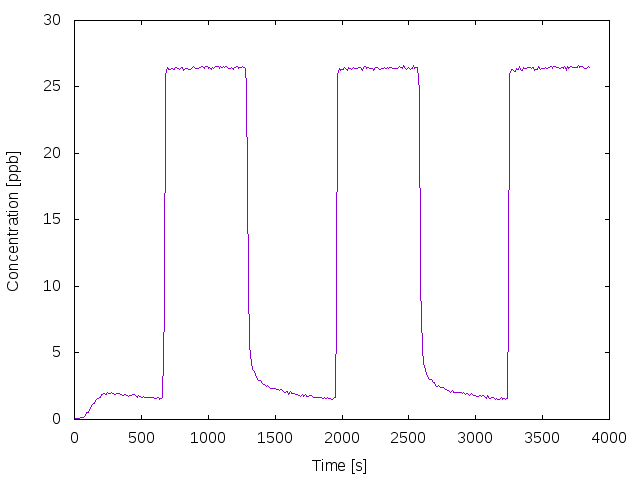
\includegraphics[width=0.7\textwidth]{20160223_15_equil_fixI0_ts.png}
  \caption{Timeseries of the measured \ch{NO2} concentration while
    switching the Ozone stream on and off.}
  \label{fig:switch}
\end{figure}
\todo{add markers for ozone switch}

\begin{figure}[htbp]
  \centering
  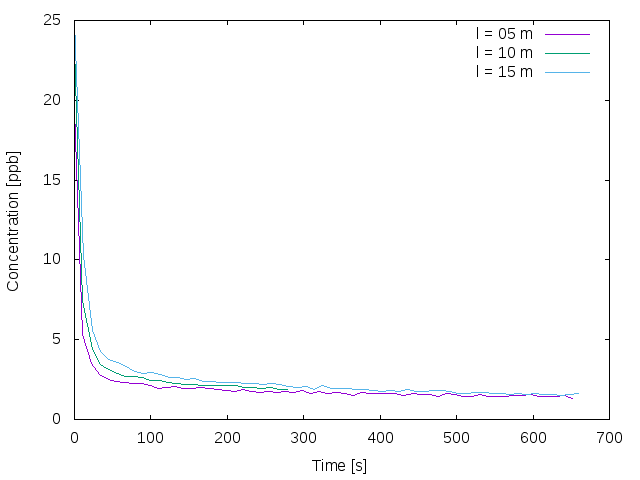
\includegraphics[width=0.7\textwidth]{20160223_equil_fixI0_fall.png}
  \caption{The behaviour of the falling flanks depending on the
    reaction pathlength}
  \label{fig:switch-pl}
\end{figure}


%%% Local Variables:
%%% mode: latex
%%% TeX-master: "../Bachelor"
%%% End:
